\documentclass{acm_proc_article-sp}
\usepackage{algorithm}
\usepackage{algorithmic}

\usepackage{amssymb}
\usepackage{amsmath}
%\usepackage{subfigure}
\setcounter{tocdepth}{3}
\usepackage{graphicx}
\usepackage{enumerate}
\usepackage{verbatim}

\begin{document}
\title{Weight-Based Personalized Recommendation using Egocentric and Collaborative Filtering}
\numberofauthors{4} 
\author{
% 1st. author
\alignauthor Vijesh M\\
       \affaddr{Student, Department of Computer Science}\\
       \affaddr{PES Institute of Technology}\\
       \affaddr{Bengaluru, India}\\
       \email{mv.vijesh@gmail.com}
% 2nd. author
\alignauthor Sandeep Raju P\\
       \affaddr{Student, Department of Computer Science}\\
       \affaddr{PES Institute of Technology}\\
       \affaddr{Bengaluru, India}\\
       \email{sandeep080@gmail.com}
% 3rd. author
\alignauthor Vijay Mahantesh SM\\
       \affaddr{Student, Department of Computer Science}\\
       \affaddr{PES Institute of Technology}\\
       \affaddr{Bengaluru, India}\\
       \email{vijaym123@gmail.com}
%\and  % use '\and' if you need 'another row' of author names
\and
% 4th. author
\alignauthor Pallavi Karanth\\
       \affaddr{Researcher}\\
       \affaddr{Department of Ontology}\\
       \affaddr{PES Institute of Technology}\\
       \affaddr{Bengaluru, India}\\
       \email{pallavik@pes.edu}
}
\maketitle
\begin{abstract}
Personalized Recommendations serve as an important ingredient for several web based systems. These systems generally house a knowledge base containing the metadata about items and users. In this paper, we present an approach for the purpose of generating personalized recommendations to users. We've developed a graph based solution that establishes relations between items and performs unsupervised dimensionality reduction on the dataset. Alongside dimensionality reduction, we perform user profiling to determine the relative importance that a particular user gives to individual attributes. We define a characteristic parameter for each user that depicts how egocenric the user is, in choosing the items to consume. We split the process of recommendation into three stages, egocentric recommendation, collaborative filtering and hybridization of the results as a weighted combination using the egocenric behavior of the user as the weight. In our experiments, we have used the MovieLens dataset 
in combination with the metadata about the movies from IMDB. For experimental purposes, we split the aggregated dataset into two parts: training set and the test set, comprising of 70 percent and 30 percent of the user data respectively. Finally, from the hybridized scores thus obtained, it is possible to predict the probable rating that a user might give to a movie. For the purpose of evaluation of the results, we use Mean Absolute Error as a metric.
\end{abstract}\\

\textbf{Keywords} : \emph{unsupervised dimensionality reduction, MovieLens dataset, Graph based egocentric recommendation and collaborative recommendation}

\section{Introduction}

The outburst of information on the Web has necessitated the development of effective techniques to automatically filter and organize content that are relevant to the users. Efforts have been put forth to automate the filtering and organization process. In this regard, many Recommender Systems have been developed and evaluated for performance and accuracy, with inherent tradeoffs. A general purpose recommender system for a web application fetches the information about the items from the user and recommends the items that the user is likely to be interested in. Till date, hundreds of sites implement recommender systems to serve their customer bases. One of the most effective techniques used in these systems is Collaborative Filtering. The scope for research in Recommendation Systems grew in the 1990s with the advent of early papers on Collaborative Filtering ~\cite{resnick, shardanand, hill}. 

Gradually, over the last decade, web systems have moved towards more personalized recommendations for enhanced user experience ~\cite{durao, fabian}. In this paper, we assume a setting where we have a single item type and each item is associated with a set of attributes. Each user is expected to have prior opinions on a set of items that the user has consumed. In real world, each user gives varied levels of importance towards various attributes of an item. This varied levels of importance is a crucial decisive factor for the user in choosing the items to consume. Naturally, the users tend to consume those items having the attribute for which the user gives a high importance. Hence, during recommendation, all the attributes cannot be treated as equals.

We implement this setting as an item graph, where each node is an item and each edge represents the relation between items, described in terms of common attribute-value pairs. We describe two approaches for recommendation: egocentric and collaborative filtering. Our approach for collaborative filtering demands the clustering of users which, in turn, depends on the similarity between users. The simple approach for Jaccard similarity is ignorant towards the properties of the items themselves. This arises the need to modify the simple Jaccard similarity to consider the properties of users and items. For the sake of simplicity, we consider a homogeneous dataset in our experiments. Ideally, the approach can also be extended to a heterogeneous set of items that share common attributes.

% Some examples like Google, Amazon, E-bay and MovieLens\\

% Define the environment\\
% This paper is concerned particularly with the setting where there is a single item of interest.\\

% A bit more detailed explanation on the way to model the setting\\

%  List a few landmark papers and quote them. Do so by reading other papers and reading references. Arrange them in chronological order.\\
% Talk about recommender systems

The sectional breakup of the paper is as follows. Section~\ref{sec:relatedWork} contains the related work. In section~\ref{sec:notions}, we introduce some of the fundamental notations that we use in the subsequent sections. Section~\ref{sec:dataset} explains the organization of the dataset that we have used. In section~\ref{sec:preparation}, we deal with the creation of reference structures. Section~\ref{sec:buidingItemGraph} explains the creation of item graph, section~\ref{sec:userProf} explains the creation of profiles for each user and section~\ref{sec:dimRed} provides a method for unsupervised dimensionality reduction for the dataset. In sections~\ref{sec:userSimilarity} and~\ref{sec:clustering}, we find the similarity between users and cluster them. We define the two approaches for recommendation in sections~\ref{sec:egocentric} and~\ref{sec:collab}, and provide a method to combine them in section~\ref{sec:hybrid}. We present the results obtained in section~\ref{sec:results} and conclude in section~\
ref{sec:conclusion}.

\section{Related Work}
\label{sec:relatedWork}
Recommendation systems have gained popularity in web based systems since the appearance of papers on collaborative filtering in the 1990s~\cite{resnick, shardanand, hill}.~\cite{resnick} explains the concept of collaborative filters. They introduce GroupLens as a system for collaborative filtering of netnews, to help people find articles they will like in the huge stream of available articles. They hypothesize that the users who have agreed on a certain aspect in the past will probably agree again.~\cite{shardanand} describes a technique for making personalized recommendations to a user based on the similarities between the interest profile of that user and those of other users. They also test and compare four different algorithms for making recommendations using social information filtering.~\cite{hill} presents an approach for collaborative recommendation where in the history of other users is used in the automation of a social method for informing choices to the user. Their results show that the 
communal history-of-use data can serve as a powerful resource for use in interfaces.

~\cite{konstan} determines the potential predictive utility for Usenet news. They develop a specially modified news browser that accepts ratings and displays predictions on a 1-5 scale. They compute the predictions using collaborative filtering techniques and compare the results with noncollaborative approaches.~\cite{breese} describes several algorithms designed for collaborative filtering, including techniques based on correlation coefficients, vector-based similarity calculations, and statistical Bayesian methods. They compare the predictive accuracy of the various methods in a set of representative problem domains.

Over the past decade, web systems have moved towards personalized recommendations for better user experience.~\cite{durao} describes a tag-based system for personalized recommendation. They propose an approach which extends the basic similarity calculus
with external factors such as tag popularity, tag representativeness and the affinity between user and tag.~\cite{fabian} investigates user modeling strategies for inferring personal interest profiles from social web interactions. They analyze individual micro-blogging activities on twitter and compare different strategies for creating user profiles based on the twitter messages.~\cite{andriy} presents a personalization algorithm for recommendation in folksonomies, which relies on hierarchical tag clusters.~\cite{sarwar} explores and analyzes different item-based collaborative techniques. They look into different techiniques for computing item-item similarities and various techniques to obtain recommendations from them.

Significant developments in learning using graph data has led to recent advances in recommendation techniques.~\cite{toine} presents a recommendation algorithm that includes different types of contextual information. They model the browsing process of a user on a movie database by taking random walks over the contextual graph.~\cite{ziyu} models personalized tag recommendation as a "query and ranking" problem. They also propose a novel graph-based ranking algorithm for interrelated multi-type objects.

\section{Notations and Notions}
\label{sec:notions}
This section describes the common notations and notions that we will be using throughout the paper. Items are a set of commodities that are intended to be consumed by users. The set of items are represented by $I$ and an individual item is represented by $i$. The set of users are represented by $U$. Each user $u$ is associated with a set of items and their corresponding ratings, $R_u = \{(i_1, r_1), (i_2, r_2), (i_3, r_3), ... (i_n, r_n)\}$. Each item is associated with a set of properties called attributes, represented by $a_i = \{a_1, a_2, a_3 ... a_n\}$. An attribute $a_p$ is associated with a set of values $v = \{v_1, v_2, v_3, ... v_n\}$. The rest of the notations that we use are explained as and when the quantities are defined.

\section{The Movielens Dataset and IMDB}
\label{sec:dataset}
To subject our algorithm to testing on real world data, we have used the dataset from MovieLens. MovieLens is a movie recommendation website, incubated at GroupLens, Department of Computer Science and Engineering at the University of Minnesota. The users are required to sign up and rate the movies in order to receive recommendations. The datasets can be downloaded from\\ \emph{http://www.grouplens.org/node/73}. The user datasets were created by randomly sampling users who have rated atleast 20 movies. In this paper, we have used the dataset with 1 Million ratings from 6000 users on 4000 movies. Within this dataset, we have selected enough users to obtain approximately 23000 ratings.

In order to obtain metadata about the movies within the dataset, we have used the API services from \emph{http://imdbapi.org/} and \emph{http://www.omdbapi.com/}. For every movie in the dataset, we issue an appropriate API call to obtain the metadata about the movie. Each movie in the aggregated movie dataset has the following attributes: MovieLens ID, IMDB ID, IMDB Rating, Genres, Language, Title, Country, Directors, Writers, Actors, Run Time, Rating Count and Year of Release. The user base constitutes a list of users, the movies that the user has rated and the corresponding rating.

In the following sections, we present a novel approach for the problem of recommendation. The task of recommending items to users is divided among two processes. The prior process involves the creation of reference structures, preprocessing of raw datasets and the deduction of characteristic parameters. The latter process involves using the reference structures and the characteristic parameters in order to recommend items to users.

\section{Preparation of Reference Structures}
\label{sec:preparation}
In this section, we explain the creation of reference structures and deduce the characteristic parameters of users and items. Throught this section, we illustrate the concepts and procedures by taking the aggregated MovieLens Dataset as an example. Note that the figures shown assert the explained concepts. They are generated using the reduced adaptations of the actual data that we use in the implementation of the algorithm.

\subsection{Building the Item Graph}
\label{sec:buidingItemGraph}
An item is associated with a number of attributes. Each of those attributes can be associated with a single value or multiple values. Consider any two items $i_1$ and $i_2$. It is likely that $i_1$ and $i_2$ have the same set of attributes, but the value(s) for those attributes differ. Higher the number of common attribute-value pairs between $i_1$ and $i_2$, more similar $i_1$ and $i_2$ are.

In order to represent such relation between the items, we use the graph data structure. Every node in the graph represents an item. The attributes of the items are mapped to the attributes of the nodes. An attribute of a node can be associated with a single value or a list of values. An edge between two nodes conveys that the two items are related. The attributes of the edges are the common attributes between the end nodes. Throughout the paper, we refer to the item graph as $G$. 

The entire item dataset $I$ is transformed into item graph $G$ by creating a node for each item $i$ and assigning the attributes $a_i$ to the created node. Each node is checked against every other node for a list of common attribute-value pairs. An edge is drawn between the two nodes if there is atleast one common attribute-value. The common attribute-value pairs is assigned as the property of the edge. Algorithm ~\ref{buidingItemGraph_algo} illustrates the procedure explained above.

Figures~\ref{node_G} and~\ref{edge_G} illustrate how $G$ is structured for the MovieLens dataset.

\begin{figure}[htp]
\centering
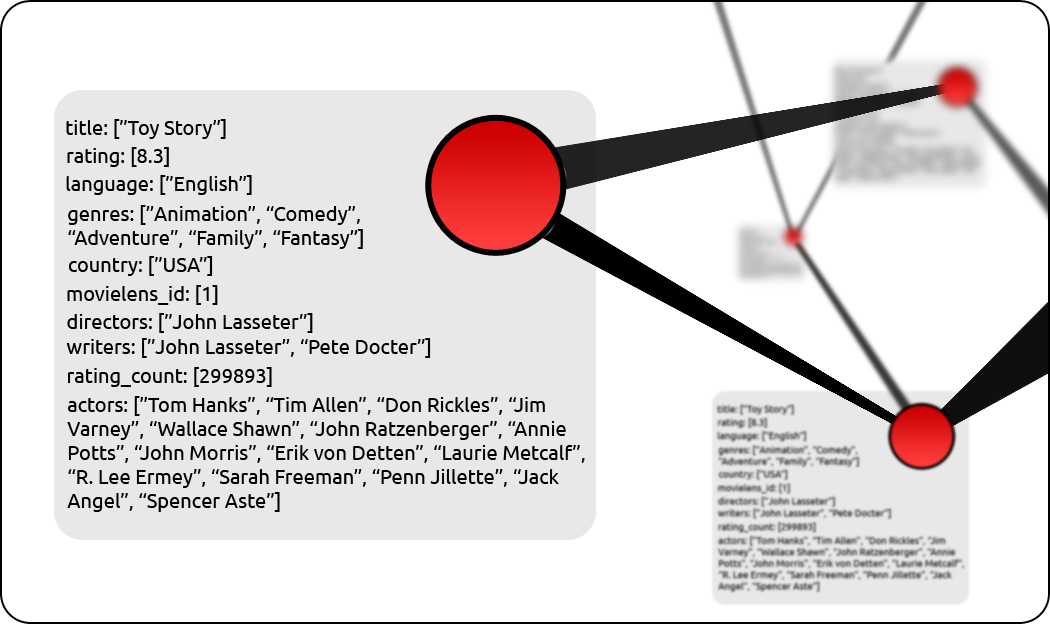
\includegraphics[scale=0.2]{Results/nodes.png}
\caption{Each item is represented by a node. The attributes of the item form the properties of the node.}
\label{node_G}
\end{figure}

\begin{figure}[htp]
\centering
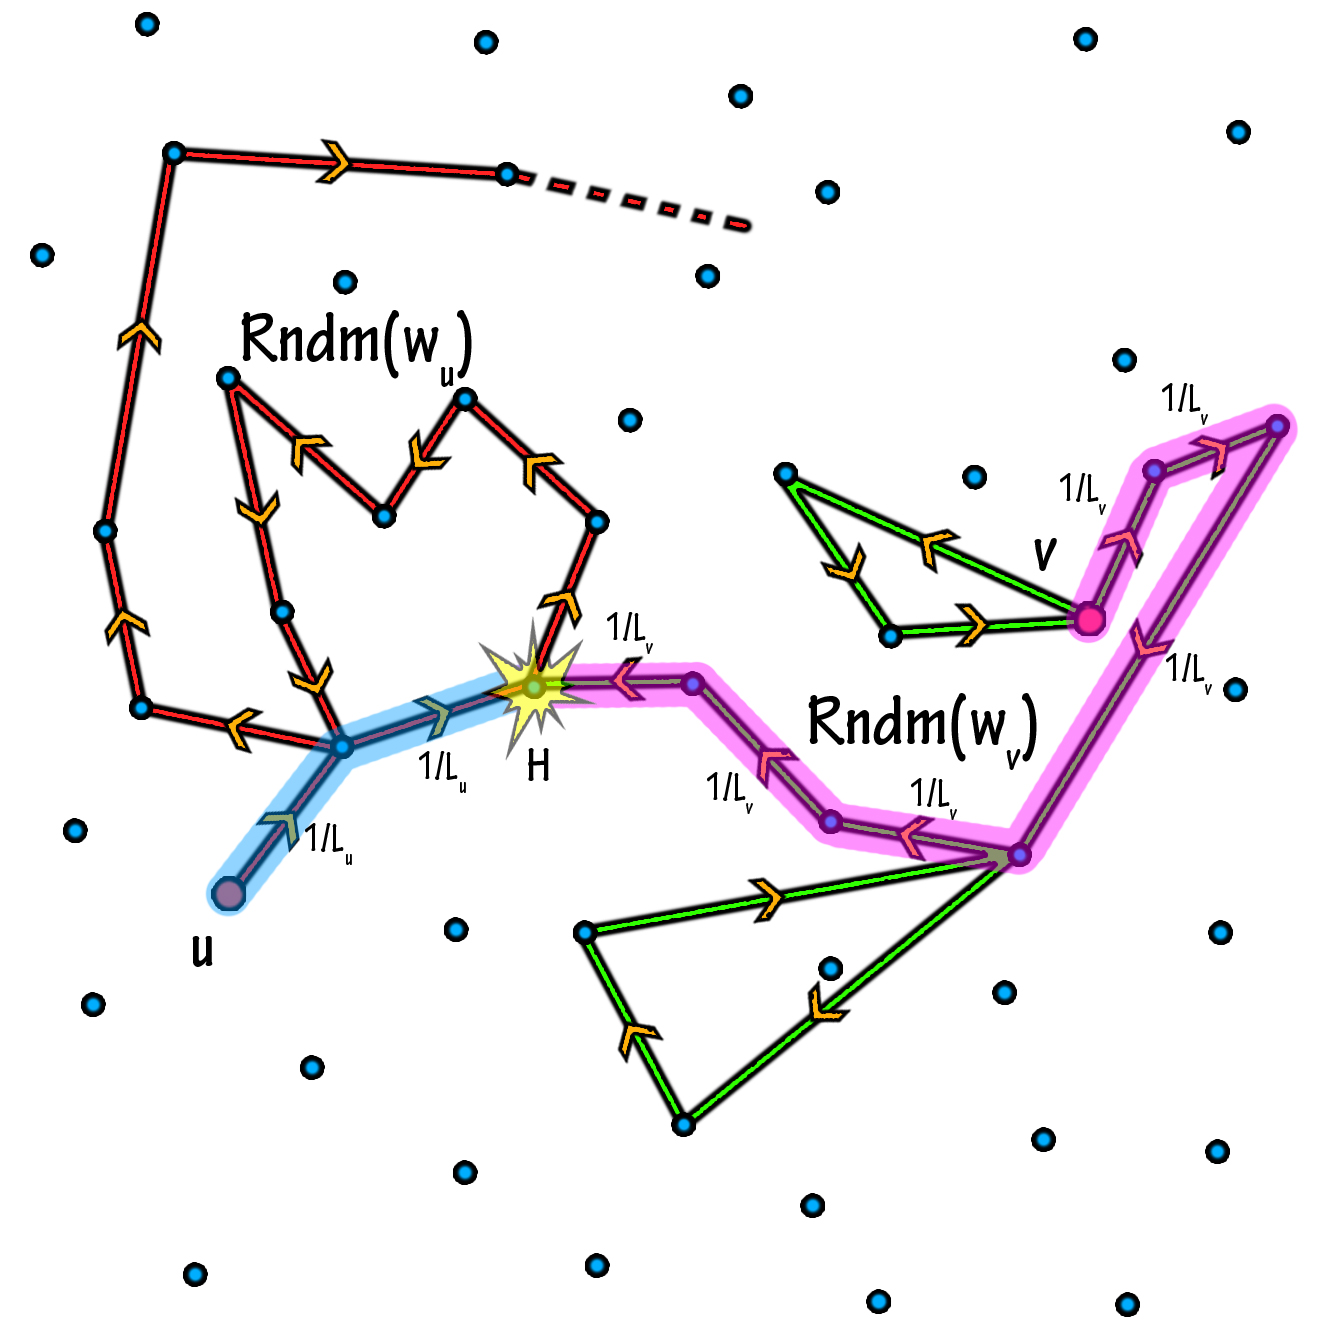
\includegraphics[scale=0.05]{Results/LearningComponent.jpg}
\caption{Items are connected to one another by edges. The attributes of the edges are the common attribute-value pairs between the end nodes.}
\label{edge_G}
\end{figure}

\begin{algorithm}
\label{buidingItemGraph_algo}
\caption{Building the Item Graph}
\begin{algorithmic}[1]
\renewcommand{\algorithmicrequire}{\textbf{Input:}}
\renewcommand{\algorithmicensure}{\textbf{Output:}}

\REQUIRE set of items $I$
\ENSURE  item graph $G(V, E)$
\STATE Initialize $G$ as an empty graph
\FORALL{items $i$ in $I$}
\STATE 
create a node $n_i$ in $G$\\
assign the attributes of the item as the attributes of the node:
$n_i \longleftarrow a_i$
 \FORALL{other nodes $n_j$ in $G$}
 \STATE
 compute common attribute-value pairs $common$
 \IF{$common \ne \phi$}
  \STATE 
  add and edge $(n_i, n_j)$ to the graph $G$\\
  set the property of edge $(n_i, n_j)$ to $common$
 \ENDIF
 \ENDFOR
\ENDFOR
\end{algorithmic}
\end{algorithm}

\subsection{Generating User Profiles}
\label{sec:userProf}
% ~\cite{stuart} search papers on user profiling\\

A user is an entity who consumes an item. In this section, we build a profile for each user. The user profile consists of characteristic parameters of the user that quantifies his behaviour.

In real world, many factors influence the decision of the user to consume a particular item. These factors include the personal choices of the user and recommendation by other users. This scenario is analogous to a customer at a restaurant. The customer might place an order due to recommendations by his friends. His decision is also influenced by what he personally prefers to eat. Generally, the customer does not have equal preferences towards all properties of the food, such as sour, salt, hot and sweet. He has varied levels of liking towards various attributes. Also, the customer might choose to place the order according to his preference or others' recommendation, with a certain probability. We generalize and quantify these behaviours of the customer in order to deduce the characteristic parameters of the customer.

It is easy to see that users behave in a similar manner, regardless of the type of item. We define two characteristic parameters associated with every user. In general, a user does not have equal preference towards all the attributes of the item. The preferences can be modeled as the weight that a user gives for each attribute of the item dataset. This forms the first characteristic parameter $w_{u_p}$. While consuming an item, the user might decide upon the item purely based on his preferences or follow others' recommendations. We define $\alpha_{u_p}$ to be the probability with which the user $u_p$ decides upon an item purely based on his preferences. $\alpha_{u_p}$ quantifies how \emph{egocentric} a user is. Closer the value of $\alpha_{u_p}$ to 1, more egocentric the user is. The user follows others' recommendation with a probability $1-\alpha_{u_p}$. This forms the second characteristic parameter.

$userProfile_{u_p} = \{w_{u_p}, \alpha_{u_p}\}$

In order to deduce the $w_{u_p}$ for a user $u_p \in U$, we construct an induced subgraph of the items that $u_p$ has rated. The properties of the edge capture the attribute-value pairs that are common between the end nodes. We hypothesize that, higher the importance that a user gives for an attribute, higher the frequency of its existance as an edge property. Conversely, the frequency of occurance of attribute as a property of the edges is proportional to the importance that the user gives. In order to determine the relative importance, we divide each frequency by the sum of frequencies.

Algorithm~\ref{userProf_algo} illustrates the methodology that we have developed to determine $w_{u_p}$ for a user $u_p \in U$.

%unsupervised learning???

\begin{algorithm}
\label{userProf_algo}
\caption{Creating User Profiles}
\begin{algorithmic}[1]
\renewcommand{\algorithmicrequire}{\textbf{Input:}}
\renewcommand{\algorithmicensure}{\textbf{Output:}}

\REQUIRE set of users, items that the user has consumed and its corresponding rating, $U$\\
item graph, $G$
\ENSURE set of user profiles, $userProfiles = \{userProfile_{u_1}, userProfile_{u_2}, ... userProfile_{u_n}\}$

\STATE Initialize an empty associative array $userProfiles$
\FORALL{user $u$ in $U$}
\STATE 
Initialize an empty associative array $D$\\ to hold the attribute and the corresponding count\\
Construct an induced subgraph $isg \in G$ of all the items that $u$ is associated with
\FORALL{edge $E \in isg$ }
 \FORALL{attribute $a \in E$}
  \IF{$D$ contains $a$}
   \STATE increment $D[a]$
   \ELSE
   \STATE $D[a] = 1$
  \ENDIF
 \ENDFOR
\ENDFOR\\
\STATE Compute the relative frequency of attributes by normalization.\\
$sum = $ sum of values of $D$
\FORALL{attribute $a$ in $D$}
\STATE $D[a] = D[a] / sum$
\ENDFOR
\STATE $userProfiles[u] = \{D, 0.5\}$
\ENDFOR
\end{algorithmic}
\end{algorithm}

Note that we have set the value of $\alpha_{u_p}$ to 0.5 for all the users initially. This is because we are still in the bootstrapping stage. We cannot determine how egocentric a user is at this stage. Such behavior can only be determined when the system is able to receive feedback from the user. Figure~\ref{attribRelFreq_user} shows the relative importance of attributes for users $2987$, $3552$ and $5997$ from the MovieLens Dataset.

\begin{figure}[htp]
\centering
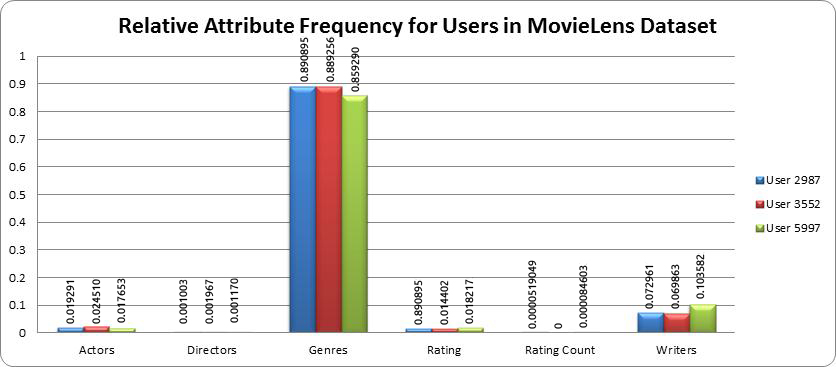
\includegraphics[scale=0.3]{Results/attribRelFreq_user.jpg}
\caption{The bar graph indicates the weights that users $2987$, $3552$ and $5997$ (from the MovieLens Dataset) have given to the corresponding attributes.}
\label{attribRelFreq_user}
\end{figure}

\subsection{Dimensionality Reduction for Items}
\label{sec:dimRed}
% ~\cite{badrul}, ~\cite{cureton}, ~\cite{deerwester}, ~\cite{berry}

Dimensionality Reduction is a well studied problem in recommender systems. Several methods, such as Latent Semantic Indexing~\cite{badrul} and Principal Component Analysis~\cite{cureton} etc, have been formulated to reduce the dimensions of the datasets. In this section, we present an empirical approach to perform dimensionality reduction on the dataset. We observe the users' pattern in consuming the items and deduce the importance of an attribute.

The importance of an attribute in the item dataset increases as number of users who give higher relative importance to that attribute increases. Hence, the importance of an attribute $a$ in the item set $I$ can be quantified as the mean relative importance of $a$, taken over all the users $u \in U$. In the previous section, we created a profile for each user. The characteristic parameter $w_{u_p}$ consists of relative weights of attributes for $u_p$. The relative importance of an attribute $a$ in the item set $I$ can be computed as follows:

$weight_a = \frac{\sum_{u_p \in U} w_{u_p}[a]}{Number\ of\ Users}$

The dimensions of the dataset can then be reduced either by thresholding or selecting the top N dimensions with highest weights. Figure~\ref{attribRelFreq_items} shows the weights for various dimensions of the aggregated MovieLens Dataset.

\begin{figure}[htp]
\centering
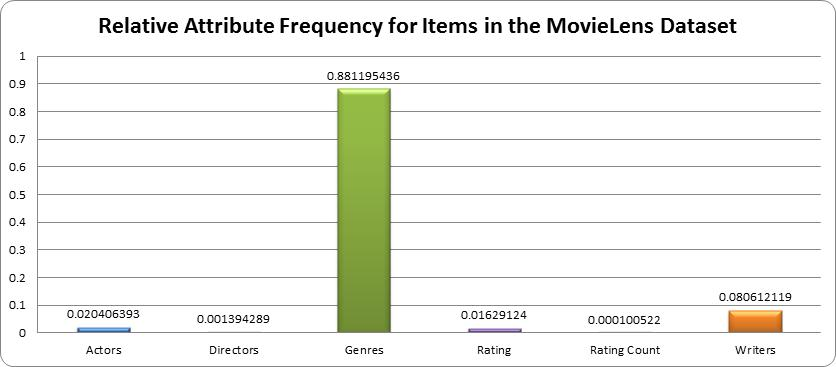
\includegraphics[scale=0.4]{Results/attribRelFreq_items.jpg}
\caption{The figure indicates the weights for various dimensions of the aggregated MovieLens Dataset, calculated using the above formula.}
\label{attribRelFreq_items}
\end{figure}

%unsupervised learning??

\subsection{Computing Similarity between Users}
\label{sec:userSimilarity}
% ~\cite{alexander}

The techniques involved in Collaborative Filtering are based on analyzing a large amount of data on users' activities and predicting what the a given user might like. The recommendations can be based on similarity between users or similarity between items. Our algorithm uses similarity between users to perform collaborative filtering. Some of the popular similarity measures are Euclidean Distance, Cosine Similarity, Pearson Correlation and Jaccard Similarity. ~\cite{alexander} presents a comparative study of the impact of these similarity measures on web page clustering.

Jaccard similarity is a measure used for comparing the similarity of sample sets. Jaccard similarity between two sets $A$ and $B$ is mathematically defined as follows:\\
$J(A,B) = \frac{|A \cap B|}{|A \cup B|}$\\
Each user is associated with a set of items that he has consumed. The similarity between users can be computed just by applying the simple Jaccard similarity between the sets of items for a pair of users. But there is an intrinsic drawback associated with this approach. The approach treats all the items to be equivalent. It is ignorant towards the properties of the items themselves and the relations between them. To include these considerations, we modify the simple formula for Jaccard similarity.

The idea behind the modification is as follows. To compute the similarity between two users $u_p$ and $u_q$, we compute two induced subgraphs of $G$. One of them contains the intersecting items of the two users, and the other contains the union of items of the two users. From the two induced subgraphs, we make two aggregated lists of edge attributes, one for each subgraph. Note that the attributes in these lists can repeat. The similarity is calculated as a fraction. To compute the numerator, we iterate  through the attributes in the aggregated list for item intersection subgraph. Counting the number of occurances of these attributes would implicitly mean that we are considering all the attribute as equals. But, the users give varied levels of importance to the attributes. Hence, for each attribute in the aggregated list, we sum up the corresponding weights from the users $u_p$ and $u_q$ and multiply the sum by the relative frequency of occurance of the attribute in the aggregated list. We follow a similar 
procedure to compute the denominator, with the only difference being that we consider the item union subgraph.

$Intrscn = [a\ |\ a \in edge\ attribute\ of\ subgraph(items\ of\ u_p\ \cap items\ of\ u_q, G)]$\\
\newline
$Union = [a\ |\ a \in edge\ attribute\ of\ subgraph(items\ of\ u_p\ \cup items\ of\ u_q, G)]$\\
\newline
$sim(u_p, u_q) = \frac{\sum (w_{u_p}[a]\ +\ w_{u_q}[a])*relFreq(a, Intrscn)\ \forall\ a\ \in\ set(Intrscn))}{\sum (w_{u_p}[a]\ +\ w_{u_q}[a])*relFreq(a, Union) \forall\ a\ \in\ set(Union))}$

where $relFreq(attrib, list)$ returns the relative frequency of occurance of $attrib$ in $list$.

Algorithm~\ref{userSimilarity_algo} illustrates the computation of similarity between all pairs of users $(u_p, u_q) \in U$. Note that $U_{sim}$ is symmetric in nature. Hence, the amount computation can be reduced approximately by half to make the implementation more efficient.

\begin{algorithm}
\label{userSimilarity_algo}
\caption{Computing User Similarity}
\begin{algorithmic}[1]
\renewcommand{\algorithmicrequire}{\textbf{Input:}}
\renewcommand{\algorithmicensure}{\textbf{Output:}}

\REQUIRE set of users, items that the user has consumed and its corresponding rating, $U$\\
item graph, $G$
\ENSURE User similarity matrix, $U_{sim}$
\STATE Number of users $N = |U|$
\STATE Initialize an empty matrix $U_{sim}$ of size $N\times N$, filled with zeros.
\FORALL{user $u_p \in U$}
  \FORALL{user $u_q \in U$}
    
    \STATE $Intersecting\_Items = $ set of intersecting items for $u_p$ and $u_q$
    \STATE $Intersecting\_Subgraph = subgraph(Intersecting_Items, G)$
    \STATE $Intersecting\_Attribs = [\ ]$
    \FORALL{edge $E \in Intersecting\_Subgraph$}
      \STATE append the attributes of $E$ to $Intersecting\_Attribs$
    \ENDFOR
    \STATE $numerator = 0.0$
    \FORALL{attribute $a$ in set($Intersecting\_Attribs$)}
      \STATE $numerator\ +=\ (\ w_{u_p}[a]\ +\ w_{u_q}[a]\ ) *$ relative frequency of $a$ in $Intersecting\_Attribs$
    \ENDFOR
    \newline
    \STATE $Union\_Items = $ set of union of items for $u_p$ and $u_q$
    \STATE $Union\_Subgraph = subgraph(Union_Items, G)$
    \STATE $Union\_Attribs = [\ ]$
    \FORALL{edge $E \in Union\_Subgraph$}
      \STATE append the attributes of $E$ to $Union\_Attribs$
    \ENDFOR
    \STATE $denominator = 0.0$
    \FORALL{attribute $a$ in set($Union\_Attribs$)}
      \STATE $denominator\ +=\ (\ w_{u_p}[a]\ +\ w_{u_q}[a]\ ) *$ relative frequency of $a$ in $Union\_Attribs$
    \ENDFOR
    
    \STATE $U_{sim}[u_p][u_q] = numerator / denominator$
    
  \ENDFOR
\ENDFOR
\end{algorithmic}
\end{algorithm}

\subsection{Clustering the Users for better Recommendation}
\label{sec:clustering}

\section{Recommendation Algorithm}
In section~\ref{sec:preparation}, we created a set of reference structures that will aid us in recommending items to users. In the subsequent sections, we will use these reference structures to recommend new items to users. We present two approaches of recommending items to users. The Egocentric approach considers only the history of the user in order to recommend new items. The Collaborative Filtering approach considers the clusters to which the user belongs and his similarity with the other users in the cluster to provide recommendation. The recommendations from both the approaches are then combined to produce a hybrid recommendation.

\subsection{Egocentric Recommendation}
\label{sec:egocentric}
% Egocentric Recommendation considers only the history of the user in order to recommend new items to the user. It does not take into consideration the relationship of the user with other users.

The egocentric algorithm works as follows. We initialize the similarity scores of all the items to zero. Given a user $u$, we analyze the list of items that $u$ has previously consumed. If a user has consumed an item $i$, it is very likely that the user might be interested to consume the neighbors of $i$, but not to equal extents. The extent to which the user might be interested to consume a neighbor not only depends upon the similarity between the items, but also upon the weight that the user gives to the common features between the items. The common features between the items are captured as the property of the edge between them. Hence, we increment the score of each neighbor by the weight that the user gives to each property of the edge. After updating all the nodes, we create an associative array of items and their score. Note that the associative array does not contain the items that are already consumed by the user. We then normalize the scores by dividing all the scores by the maximum score. The 
pseudocode for the algorithm is presented in Algorithm~\ref{egocentric_algo}.

\begin{algorithm}
\label{egocentric_algo}
\caption{Egocentric Recommendation}
\begin{algorithmic}[1]
\renewcommand{\algorithmicrequire}{\textbf{Input:}}
\renewcommand{\algorithmicensure}{\textbf{Output:}}

\REQUIRE user $u$\\
item graph $G$\\
user base $U$\\
\ENSURE Items and their corresponding egocentric scores, $scores\_ego$

\STATE Initialize the similarity scores of all the nodes in $G$ to 0.
\FORALL{item $i \in U[u]$}
  \FORALL{neighbors $n_i$ of $i$ in $G$}
    \FORALL{attribute $a$ of edge ($n_i$, $i$)}
      \STATE Increment the score of $n_i$ by $w_u[a]$
    \ENDFOR
  \ENDFOR
\ENDFOR
\STATE Initialize an empty associative array, $scores\_ego = \{ \}$ 
\FORALL{node $i \in G$ and $i \notin U[u]$}
  \STATE $scores\_ego[i] =$ similarity score of the node $i$
\ENDFOR
\STATE Normalize the scores by dividing all the scores by the maximum score
\STATE Sort $scores\_ego$ in the decreasing order of scores
\end{algorithmic}
\end{algorithm}

% On sorting $scores\_ego$ in the decreasing order, we get a pure egocentric recommendation list. In the next subsection, we describe the methodology to obtain a similar list using Collaborative Filtering techniques. It is possible to combine the obtained list with $scores\_ego$ to get a hybrid recommendation. We describe two methods of combining the lists in section~\ref{sec:hybrid}.

\subsection{Collaborative Filtering based on User Similarity}
\label{sec:collab}
Collaborative Filtering(CF) is a collection of techniques that are used in recommending items to users based on the ratings of other users. CF techniques are by far the most successful techniques in recommending items to users. The core idea behind CF techniques is the concept of similarity. The recommender systems generally use two forms of similarities: user-based similarities[quote something] and item-based similarities[quote something]. These techniques generally use a standard metric, such as Euclidean Distance, Cosine Similarity, Pearson Correlation or Jaccard Similarity[quote something]. Once a similarity matrix is build, these systems use various algorithms to generate recommendations. 

In this paper, we have used an extended version of Jaccard similarity, as described in section~\ref{sec:userSimilarity}. The algorithm that we have developed uses user-based similarity. Our algorithm begins by iterating through all the clusters. A cluster houses many users. Each user is associated with a list of items that he has consumed. For each user $u_p$ in each cluster $c$, we increment the score of each item $i$ consumed by $u_p$, by the similarity between $u$ and $u_p$. Note that the clusters we obtained are overlapping. That is, a single user can belong to multiple clusters. If the given user $u_1$ is very similar to another user $u_2$, then $u_2$ will appear in majority of the clusters where $u_1$ is present. This implies that the score for the items consumed by $u_2$ is naturally boosted, since $u_2$ is presented in most of $u_1$'s clusters and the similarity between $u_1$ and $u_2$ is high. The pseudocode for the algorithm is presented in Algorithm~\ref{collab_algo}.

\begin{algorithm}
\label{collab_algo}
\caption{Collaborative Recommendation based in User Similarity}
\begin{algorithmic}[1]
\renewcommand{\algorithmicrequire}{\textbf{Input:}}
\renewcommand{\algorithmicensure}{\textbf{Output:}}

\REQUIRE user $u$\\
item graph $G$\\
user base $U$\\
similarity matrix $U_{sim}$\\
clusters $C$\\
\ENSURE Items and their corresponding CF scores, $scores\_collab$

\STATE Initialize the similarity scores of all the nodes in $G$ to 0.
\FORALL{cluster $c \in C$}
  \FORALL{user $u_p \in c$}
    \FORALL{item $i \in U[u_q]$}
      \STATE Increment the score of $i$ by $U_{sim}[u][u_p]$
    \ENDFOR
  \ENDFOR
\ENDFOR
\STATE Initialize an empty associative array, $scores\_collab = \{ \}$ 
\FORALL{node $i \in G$ and $i \notin U[u]$}
  \STATE $scores\_collab[i] =$ similarity score of the node $i$
\ENDFOR
\STATE Normalize the scores by dividing all the scores by the maximum score
\STATE Sort $scores\_collab$ in the decreasing order of scores
\end{algorithmic}
\end{algorithm}

On sorting $scores\_ego$ and $scores\_collab$ in the decreasing order, we get a pure egocenric recommendation list and a pure collaborative recommendation list respectively. In the next subsection, we describe a method to combine $scores\_ego$ and $scores\_collab$ to get a hybrid recommendation.

\subsection{Hybrid Recommendation}
\label{sec:hybrid}
Sections~\ref{sec:egocentric} and~\ref{sec:collab} dealt with generating egocentric and collaborative recommendations for the user. Both the algorithms associated a real number between 0 and 1 with each item that a user has not consumed. Hybrid Recommendation involves combining $scores\_ego$ and $scores\_collab$ into a single list $scores\_hybrid$, by means of weighted combination of corresponding items from both the lists.

Since we are merging the lists that signify egocentric behavior and group behavior, we choose $\alpha_{u_p}$ as the weight. In section~\ref{sec:userProf}, we had defined $\alpha_{u_p}$ as the probability with which the user $u_p$ decides upon an item purely based on his preferences. $\alpha_{u_p}$ quantifies how \emph{egocentric} a user is. Hence, assign a weight $\alpha_{u_p}$ to $scores\_ego$ and $1 - \alpha_{u_p}$ to $scores\_collab$.

We propose two methods by which the lists can be combined:
\begin{enumerate}
 \item Rank based weighted average:\\
 In this approach, we take a weighted average of ranks of each item and sort the items in the decreasing order of their composite ranks. As mentioned earlier, we assign a weight $\alpha_{u_p}$ to $scores\_ego$ and $1 - \alpha_{u_p}$ to $scores\_collab$. The following formula mathematically describes the operation:\\
 $compositeRank_i = \alpha_{u_p}*rank(i, scores\_ego) + (1 - \alpha_{u_p})*rank(i, scores\_collab)$
 
 \item Score based weighted average:\\
 In this approach, we take a weighted average of score of each item and sort the items in the decreasing order of their composite scores. As mentioned earlier, we assign a weight $\alpha_{u_p}$ to $scores\_ego$ and $1 - \alpha_{u_p}$ to $scores\_collab$. The following formula mathematically describes the operation:\\
 $compositeScore_i = \alpha_{u_p}*scores\_ego[i] + (1 - \alpha_{u_p})*scores\_collab[i]$
\end{enumerate}

Rank based weighted average method can be used to provide recommendations to the user in the order of their ranks. But predicting the rating that the user might give to an item tends to be relatively hard. Consequently, evaluating the accuracy of our algorithm also tends to be relatively hard. Hence, in our experiments, we use the score based weighted average method to predict the rating that a user might give to a new item.

%As an alternative approach, we could let the user set the value of alpha.

\section{Results and Discussions}
\label{sec:results}
\subsection{Dataset}
As mentioned in section~\ref{sec:dataset}, we have used the aggregated MovieLens Dataset in our experiments. We have used the dataset with 1 Million ratings from 6000 users on 4000 movies, and retrieved the metadata about the movies from\\
\emph{http://imdbapi.org/} and \emph{http://www.omdbapi.com/}. We split the user dataset into two parts, training data and test data. The training data constitutes 70 percent of the dataset. The users in the training set were chosen randomly. We test the accuracy of our algorithm by predicting the user ratings in the remaining 30 percent of the dataset.

\subsection{Evaluation Metric}
% Evaluation of Recommender Systems, Resnik et al 1994
% Evaluating Collaborative Recommender Systems, Jonathan L. Herlocker
% Evaluating Recommendation Systems, G Shani, A Gunawardhana, Recommender Systems Handbook, 2011, Springer

The performance of recommender systems have been extensively studied in research literature since 1994~\cite{resnick}.~\cite{jonathan} broadly classifies recommendation accuracy metrics into three classes: predictive accuracy metrics, classification accuracy metrics and rank accuracy metrics. In this paper, we have chosen to evaluate our algorithm using a type of predictive accuracy measure called \emph{Mean Absolute Error} (MAE). It measures the average absolute error in the predicted rating and the user's true rating.~\cite{breese, shardanand} present some of the cases where MAE has been used to evaluate recommender systems. MAE is mathematically defined as follows:\\

$|E| = \frac{\sum_{i=1}^{N}|p_i - r_i|}{N}$

\subsection{Experimental Results}
In this section, we present the results obtained on applying our algorithm to the aggregated MovieLens Dataset. Section~\ref{sec:buidingItemGraph} dealt with the creation of item graph $G$. Figure~\ref{movielens_itemGraph} is a snapshot of the item graph $G$. Given two movies from the dataset, just a single common attribute-value pair will result in an edge formation. Hence, the graph that we obtain is fairly dense. After transforming the aggregated MovieLens dataset, we found that $G$ was a very dense graph, with a density of 0.47435, with an average degree of 1842.41.

% Figures~\ref{node_G} and~\ref{edge_G} show a more elaborate view of the structure of $G$.
% 
% \begin{figure}[htp]
% \centering
% 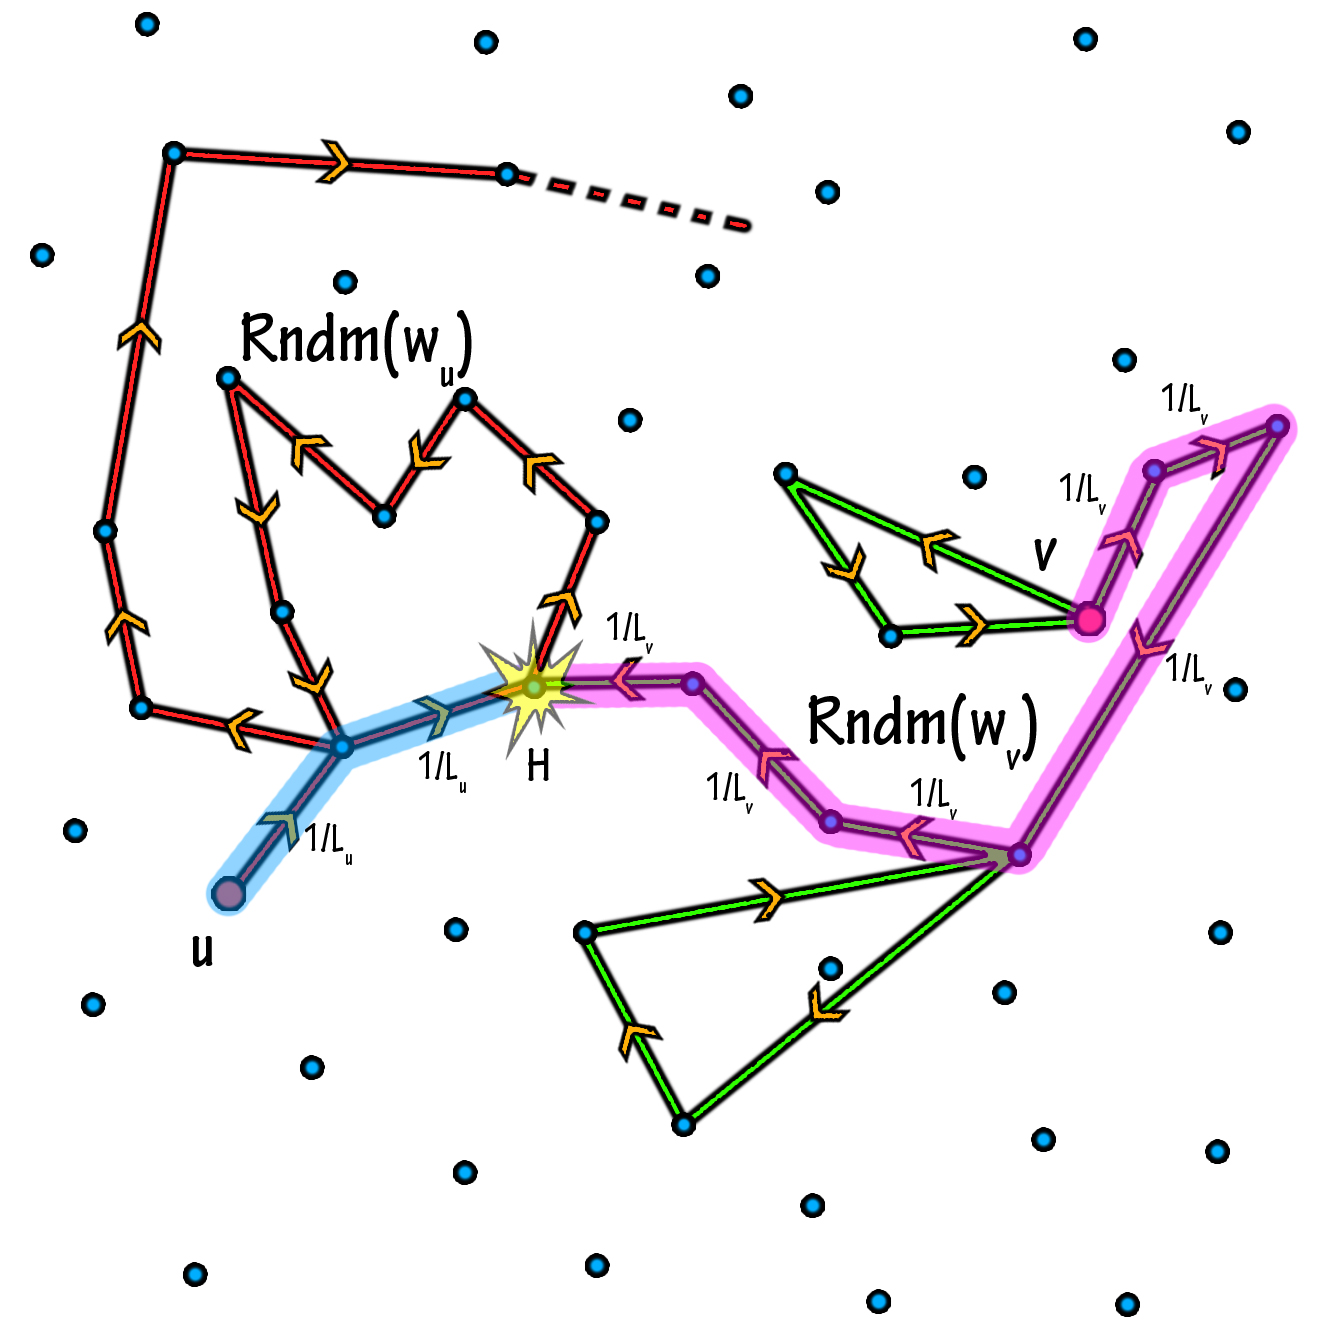
\includegraphics[scale=0.05]{Results/LearningComponent.jpg}
% \caption{Snapshot of $G$. The graph is built using the aggregated MovieLens dataset}
% \label{movielens_itemGraph}
% \end{figure}

In section~\ref{sec:userProf}, we created the profiles for each user, $userProfile_{u_p}$. We also defined two characteristic parameters, $w_{u_p}$ and $\alpha_{u_p}$, for each user. We provided a methodology to determine $w_{u_p}$ in Algorithm~\ref{userProf_algo}.

Figure~\ref{movielens_attrRelFreq_user} statistically illustrates the weights for the user $2987$ of the MovieLens dataset, for various attributes. In general, it is very likely that the users watch the movies from the same country that they reside in. As far as the dynamics of shooting movies go, the filming locations of a movie are likely to be in the same country that the movie is being produced. In general, users who are familiar with a particular language tend to watch the movies from the same language. Naturally, the weights for country, filming locations and language are relatively high. The fact that there are comparitively limited number of values for a particular also boosts up the relative score. The ratio between relative scores indicates the number of times that a particular attribute is important, relative to the other. From the figure, we can deduce that the user $2987$ statistically gives $37.3$ times more importance to actors, compared to directors. On similar lines, user $2987$ gives 3.5 
times more importance to genre, compared to actors.

\begin{figure}[htp]
\centering
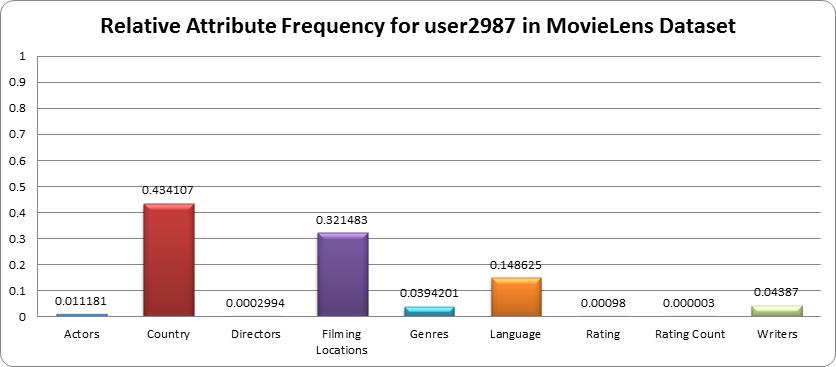
\includegraphics[scale=0.38]{Results/movielens_attrRelFreq_user2987.jpg}
\caption{Relative Attribute Importance for the user $2987$ of the MovieLens dataset}
\label{movielens_attrRelFreq_user}
\end{figure}

In section~\ref{sec:dimRed}, we reduced the dimensionality of the dataset based on the relative importances that each user gives to a particular attribute. We apply the same techinique to the aggregated MovieLens dataset. Figure~\ref{movielens_attrRelFreq_item} shows the relative attribute importance for the dataset.

\begin{figure}[htp]
\centering
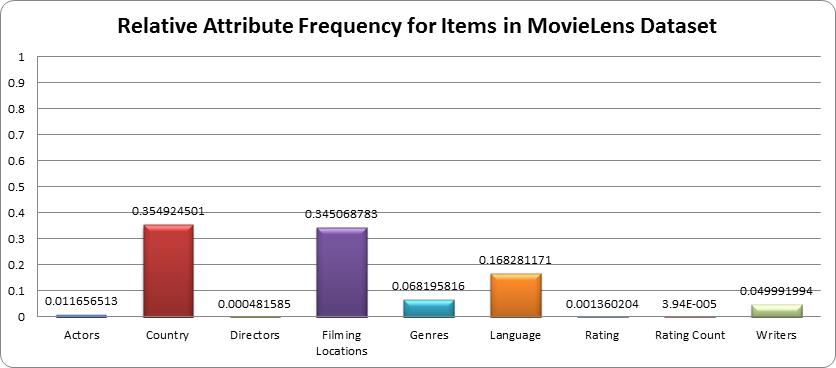
\includegraphics[scale=0.38]{Results/movielens_attrRelFreq_item.jpg}
\caption{Relative Attribute Importance of the items in the MovieLens dataset}
\label{movielens_attrRelFreq_item}
\end{figure}

We analyze the data for the entire aggregated MovieLens dataset in the same way as we did for user $2987$. On an average, we find that the users statistically give $24.2$ times more importance to actors in comparison with directors. On similar lines, users give $5.8$ times more importance to genres, compared to actors.

% In section~\ref{sec:userSimilarity}, we modified the simple Jaccard similarity to include information about the items and user preferences as well. In section~\ref{sec:clustering}, we classified the users into overlapping clusters.

% <visualization of cluster??? yes if possible>

To evaluate the accuracy of our algorithm, we use MAE as the evaluation metric. We use $\alpha_{u_p}$ as a parameter in our experiments. For varying values of $\alpha_{u_p}$, we predict each user's ratings for all the movies that the user has not rated in the training set. We compare these predicted ratings with the actual ratings present in the test set and compute the MAE. The variation of MAE for various values of $\alpha_{u_p}$ is shown in Figure~\ref{movielens_mae_alpha}.

\begin{figure}[htp]
\centering
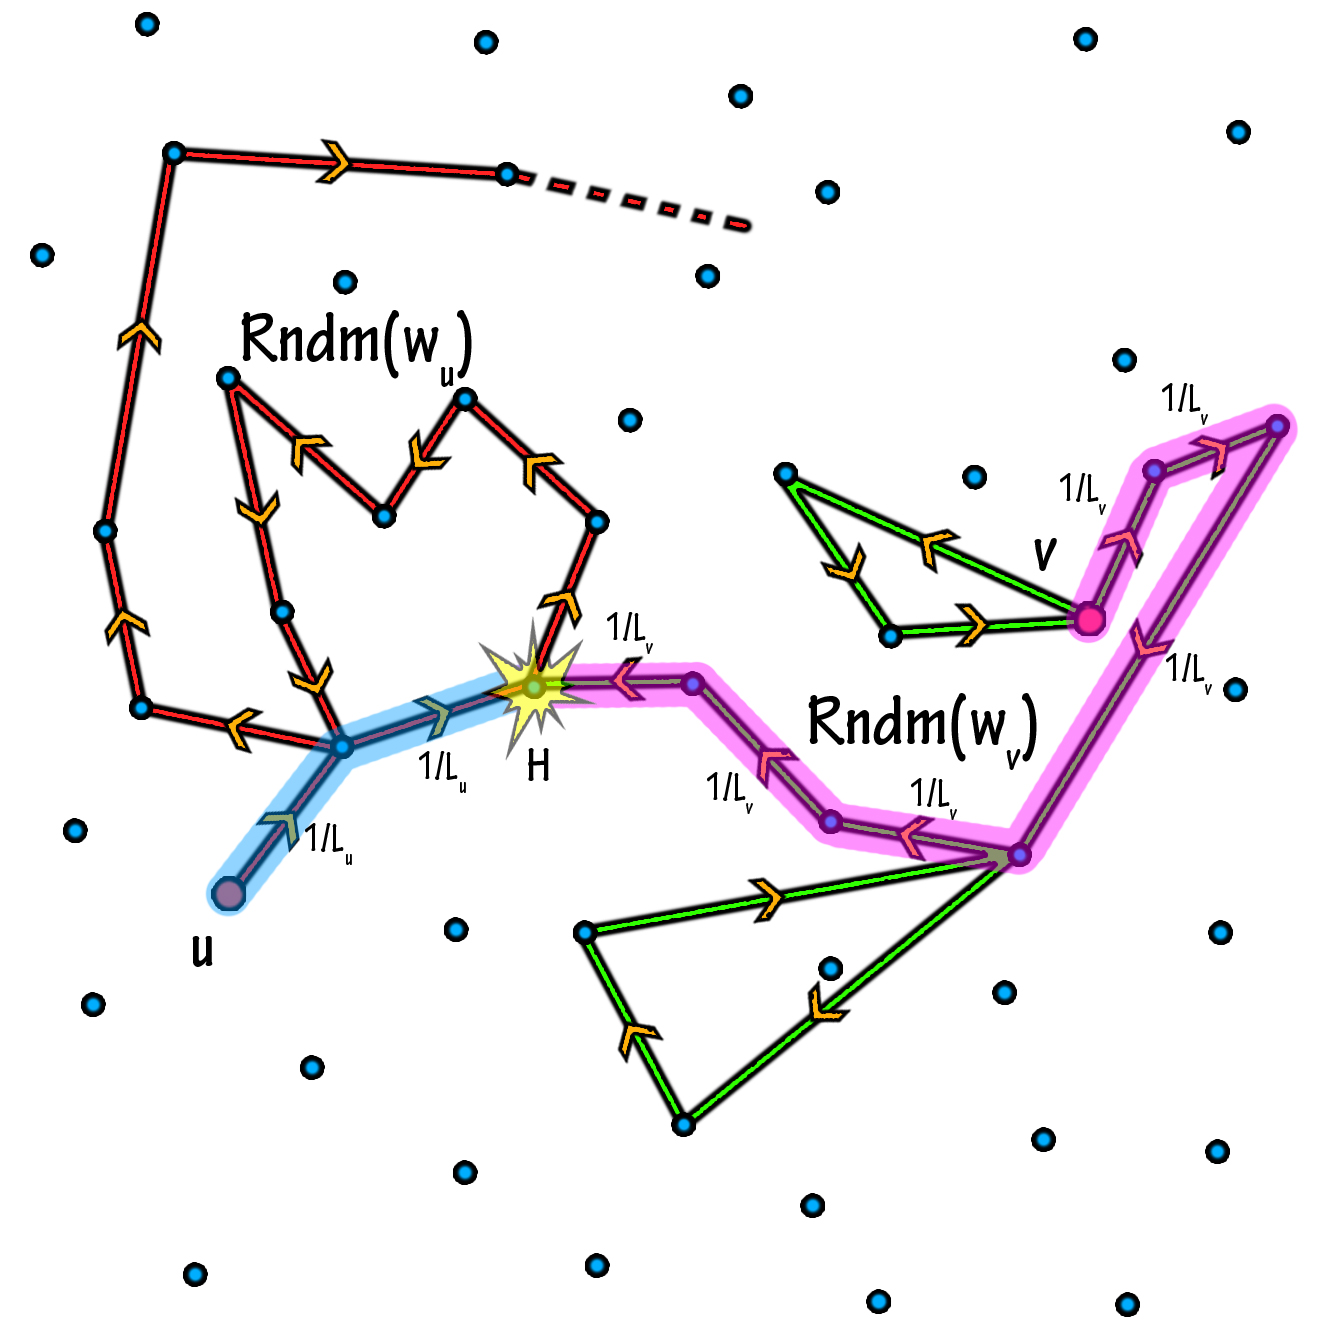
\includegraphics[scale=0.05]{Results/LearningComponent.jpg}
\caption{The plot of variation of Mean Absolute Error with varying values of $\alpha_{u_p}$}
\label{movielens_mae_alpha}
\end{figure}

Explain what happens at extreme points, i.e, at $\alpha_{u_p} = 0$ and $\alpha_{u_p} = 1$

% refer to the dataset explanation
% refer to figure with nodes and edges - for building graph
% sample diagram with weights for attributes for multiple users
% 
% describes our experimental work
% details of our dataset, evaluation metrics, methodology, results of different experiments and discussions.

\section{Conclusion}
\label{sec:conclusion}
In this paper, we demonstrated a novel approach for recommending items to users and performed experiments on the aggregated MovieLens dataset to test our algorithm. We use graph as the core reference structure. We form a graph of items and the relations between items are manifested as properties of the corresponding edges. Based on the users' history of item consumption, we profile each user and deduce the weight that the user gives to the attributes. We use the profiles to statistically determine the importance of each attribute in the dataset, in turn performing dimensionality reduction. To find out the similarity between users, we modified the simple Jaccard similarity to consider the properties of users and items. Based on a similarity threshold, we form overlapping clusters of users. To provide recommendation for a particular user, we follow two distinct approaches: egocentric and collaborative filtering. These recommendations are then combined to form hybrid recommendation.

Our results show that the importance of each dimension of the dataset can be weighted in an unsupervised manner, in accordance with the pattern that the users follow to consume the items. We deduce the relative importance that each user gives to each of the attributes. The recommendations that we provide to a user is personalized based on the corresponding relative importances of the corresponding user. We also show the variation in the Mean Absolute Error of our rating predictions as we increase the egocentric behavior of the user.

\section{Future Work}
Our experiments were performed on the MovieLens dataset of an intermediate size, with a restricted number of ratings and users. The tests must be performed on larger datasets, with a wide variety of attributes. The characteristic parameter $\alpha_{u_p}$ represents how egocentric a user is. Determining the value of this parameter calls for a feedback mechanism from the users. At the time of the writing, we are designing the methods to obtain this parameter.

In this paper, we have presented the empirical results that we have obtained on applying our algorithm on the dataset. The theoritical bounds of the algorithm is yet to be formulated. The approach presented in this paper does not enforce all the items to have the same set of attributes, i.e, the attributes need not be homogeneous across all the items. In our experiments, we have chosen a homogeneous dataset. The tests must be performed on heterogeneous datasets, where it is not necessary that all items have the same set of attributes.\\

\section{Acknowledgements}
The work was conducted at PES Institute of Technology, West Campus, Bengaluru, India. We would like to thank Ms. Pallavi Karanth, for her guidance. We would also like to thank Dr. Kavi Mahesh, for strengthening our understanding of the subject. We would also like to thank Prof. Nitin V Pujari, HOD, Department of Computer Science, PESIT and Dr. KNB Murthy, Principal, PESIT for providing us with an opportunity to carry out the research work. We also thank anonymous reviewers for their valuable comments.

\bibliographystyle{plain}
\bibliography{references}

\end{document}